\chapter{Getting Started}

In this chapter we will explain what ImageJ macros are, what you can do with them and what limitations they have. In order to be able to write macros will install FIJI. FIJI\cite{schindelin_fiji:_2012} stands for ''FIJI is Just ImageJ''. FIJI is a distribution of ImageJ that comes with a number of extensions (plugins and macros) for biological-image analysis. 

\section{Macros}

In ImageJ, macros are scripts, written in the ImageJ-macro language\cite{mutterer_macro_2010}, that can be executed by ImageJ and that allow to automatize most of the things that you can manually with ImageJ. All entries in the ImageJ menus can be called from a macro. Furthermore the macro language provides some basic data types like numbers and strings and basic programming constructs like loops and conditional execution. Finally it provides an interface to ImageJ's objects and tools like images, files, histograms, regions of interest (roi), the roi-manager, the curve fitting tool, overlays and more. 

Macros can run completely without user interaction (in batch mode) or with user interaction. A macro can have a simple user interface that allows to adjust parameter values. Macros can be integrated into ImageJ as ImageJ menu commands or as tool buttons. They can be run from the command line of your operating system or from ImageJ and they can be triggered from events like the opening of a new image in ImageJ. They can even be run from within other software packages like Cellprofiler\cite{lamprecht_cellprofiler:_2007} or KNIME\cite{berthold_knime_2009}.

ImageJ allows the usage of other scripting languages. The standard ImageJ distribution comes with JavaScript as scripting language and FIJI has support for JavaScript, Jython, JRuby, Clojure and BeanShell. What is the difference between these scripting languages and the ImageJ-macro language? Technically the ImageJ macro language is interpreted by ImageJ while the other languages are either interpreted by a special java program or compiled into java-bytecode that is executed by the java virtual machine. The world macro is an abbreviation for macroinstruction. In assembler and other programming languages macroinstructions are used as a shorthand for multiple basic instructions. The macro is replaced by a pre-processor by the basic instructions. In a similar way ImageJ's macro language can be thought of as allowing to bundle a number of basic ImageJ commands, give them a name and allow to run them using that name or by a keyboard shortcut. This point of view is supported by the fact that ImageJ macros can be created by recording the menu commands called  in an interactive ImageJ session. However it has some elements that go beyond usual macro languages mainly the ability to define functions and to call them recursively, which means that a function can directly or indirectly call itself with eventually modified parameters and the execution repeats until a condition is fulfilled. The main difference is in the complexity. The ImageJ macro language is build to provide enough glue to automatize ImageJ. The scripting languages are general purpose programming languages that can access ImageJ's application user interface. They are therefore more complex and more difficult to learn. However the minimalism of the macro language comes with a price. Although beginners will easily get started with it, more advanced things might be harder to do. Another problem is the limited re-usability of macros. Since there is no import or include statement for macros, functions must be defined in each macro. The only way to make a function available in multiple macros is to make it available to all macros.

ImageJ allows to write plugins in the java programming language as well. As a difference from macros and scripts these plugins need to be compiled and installed before they can be run. 

As a conclusion from the above, the ImageJ macro language is certainly a good choice if you want to automatize an analysis protocol that you can execute manually with ImageJ. If you need to implement complex new image analysis algorithms, scripting languages or plugins might be a better choice.         

\section{Installing Fiji}

Download the version of Fiji appropriate for your operating system from \url{http://fiji.sc/Downloads}. Unzip the archive file and save the containing folder {\tt Fiji.app} into a directory for which you have write access. Enter the folder {\tt Fiji.app} and run the application by double-clicking the program that starts with {\tt ImageJ-}. By default FIJI will check for updates each time you start it. If updates are available, accept the check and apply the changes.

\begin{figure}[h!]
  \centering
    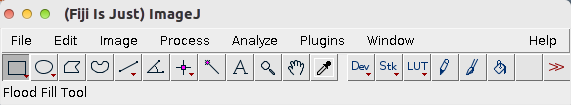
\includegraphics[width=0.85\textwidth]{fiji_launcher}
    \caption[The FIJI launcher window]{The FIJI launcher window.}
    \label{fiji_launcher}
\end{figure}

\section{Hello World}

We will now write the traditional ''Hello World!'' example. The idea is that whenever you start to learn a new programming language you first write a very simple program that outputs the text ''Hello World!''. This allows you to learn how to edit and run programs in the new language and programming environment.

We will write three different versions. One that does the output in a log-window, another that writes the output on a dialog and a last one that writes the output into a new image.

\subsection{Hello World using the log-window}

Open the macro-editor from the menu {\tt Plugins>>New>>Macro}. The macro-editor will open on a new macro with the name {\tt Macro.ijm}. The file-extension {\tt .ijm} stands for \textbf{i}mage\textbf{j} \textbf{m}acro. In the editor window enter the following command:

\begin{listing}[H]
\begin{minted}[frame=lines]{java}
print("Hello World!");
\end{minted}
\caption{Hello World using the log-window.}
\label{lst:hello_world_log_window}
\end{listing}
 
Execute the macro from the menu {\tt Run>Run} or by pressing {\tt ctrl+r}. If the log window was closed it will be opened. The text ''Hello World!'' will be written to the log window each time you run the macro. 

\begin{figure}[h!]
  \centering
    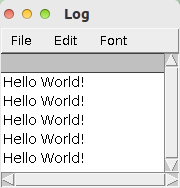
\includegraphics[width=0.4\textwidth]{log_window}
    \caption[A message in the log window]{The ''Hello World'' message displayed in the log window.}
    \label{log_window}
\end{figure}

Now let us examine the macro from listing \ref{lst:hello_world_log_window} in detail:
\begin{itemize}
\item {\tt print} is a build in function of the ImageJ macro language that allows to write output somewhere. By default the output is written to the log window.
\item the brackets separate the name of the function from the argument or the arguments that are passed to the function
\item ''{\tt Hello World!}'' is a literal string. A string is a sequence of characters. It is literal because the characters are directly written down. The macro language knows that it is a literal string and not a misspelled command because it is embedded within the '' characters.
\item the semicolon is necessary to separates commands in a macro (since this macro only has one command it would run without the semicolon at the end).
\end{itemize}

\subsection{Hello World using a dialog}
	
Either open the macro editor again from the menu {\tt Plugins>>New>>Macro} or if it is still open, open a new macro in the editor from the menu {\tt File>>New} of the editor window. This will open a second tab for the new macro. This time enter the command:

\begin{listing}[H]
\begin{minted}[frame=lines]{java}
showMessage("Hello World!");
\end{minted}
\caption{Hello World using a dialog.}
\label{lst:hello_world_dialog}
\end{listing}

Run the macro. It will show the ''Hello World!'' message on a dialog. Note that the dialog is modal. While it is open the execution of the macro is paused and all other windows of ImageJ are unresponsive. This makes sure that the user notices the message before he continues working. You can close the dialog by pressing the ''OK'' button.

\begin{figure}[h!]
  \centering
    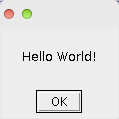
\includegraphics[width=0.2\textwidth]{hello_world_dialog}
    \caption[A message on a dialog]{The ''Hello World'' message displayed on a dialog.}
    \label{dialog_window}
\end{figure}

If you want to know more about the {\tt print} or the {\tt showMessage} commands, call {\tt Help>Macro Functions...} from the ImageJ launcher window. This will open a description of all build in functions of the macro language.

\subsection{Hello World on an image}

Since this workshop is about image analysis, we will now display the ''Hello World!'' message on an image. We will do this in a way that does not modify the pixel values of the image, by using an overlay. We will use the example to introduce the macro-recorder and to show how to run single macro commands.

Open an image. ImageJ comes with a number of example images. You can use one of those, for example the ''Fluorescent Cells'' image. Download it via the menu item {\tt File>>Open Samples>>Fluorescent Cells (400K)}. Open the macro-recorder from {\tt Plugins>>Macros>>Record...}. Any command you run will be recorded by the macro recorder now, until you close the ''Recorder'' window. In order to write the text we use the text tool. It is the 9th tool-button on the ImageJ launcher window (the one labelled 'A'). Note that double clicking the button opens a dialog that allows to modify the options of the text tool. Select the text tool, click somewhere in the image and open a rectangular selection. Type in ''Hello World!''. When done use {\tt Image>>Overlay>>Add Selection...} to add the text to an overlay or press {\tt ctrl+b}. Click somewhere in the image to get rid of the selection and see the effect of adding the text to the overlay. We're done, now let us create the macro from the recorded commands. On the macro-recorder, press the 'Create' button. This will open the macro editor with the list of recorded commands copied into it.

\begin{listing}[H]
\begin{minted}[frame=lines, linenos]{java}
//setTool("text");
setFont("Serif", 40, " antialiased");
setColor("#ffc800");
Overlay.drawString("Hello World!", 126, 128, 0.0);
Overlay.show();
\end{minted}
\caption{A macro that writes ''Hello World!'' onto an overlay of an image.}
\label{lst:hello_world_image}
\end{listing}

Remove the overlay you created when you recorded the macro by using {\tt Image>>Overlay>>Remove Overlay}. Now run the macro and make sure it reproduces the ''Hello World!'' message.

\begin{figure}[h!]
  \centering
    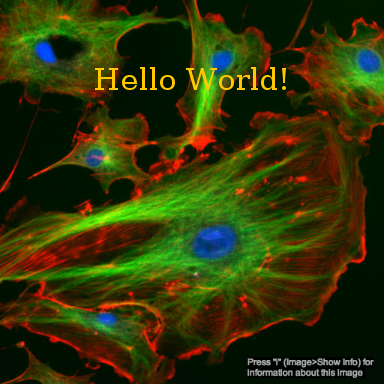
\includegraphics[width=0.4\textwidth]{Hello_World_Result}
    \caption[A text displayed on an image]{The ''Hello World'' message displayed on an overlay of an image.}
    \label{hello_world_result}
\end{figure}

We will examine the macro step by step again:
\begin{enumerate}
\item the line beginning with two slashes is a comment. In this case the macro-recorder added it to record that the text tool has been activated. It uses a comment because the selection of the text tool will not modify the result of the macro. You can remove this line from your macro.
\item {\tt setFont} is a build in function that sets the font for the {\tt drawString} function.
\item {\tt setColor} sets the foreground color. The foreground color will be used by the {\tt drawString function}. However it is used for other purposes as well and it would be a good idea to reset it after the macro. Colors can either be passed by name (''black'', ''blue'', ''cyan'', etc.) or by a hexadecimal representation of the rgb-values (''\#ff0000'' is pure red, ''\#00ff00'' pure green, etc.)  
\item the {\tt drawString} function of the Overlay takes the string to draw, the location on the image and the angle in which the text will be drawn as input.
\item the {\tt show} function of the Overlay makes the overlay visible on the image.
\end{enumerate}

We will now hide and show the overlay by running single macro commands. Just before the line {\tt Overlay.show()} insert another line and type {\tt Overlay.hide()}. Use the mouse to select the newly inserted line and call {\tt Run>>Run selected code} from the menu or press {\tt shift+ctrl+r}. The overlay becomes invisible. Make it visible again by selecting and executing the next line of the macro.

Another way to run single macro commands is to use the Macro interpreter. You can open it from {\tt Plugins>>Scripting>>Macro Interpreter}. In the lower part type {\tt Overlay.hide()} and press {\tt enter}. The command will be executed. Now type {\tt Overlay.show()} and press {\tt enter}. Note that you can use the up and down arrow keys on your keyboard to select previously executed commands.

\begin{figure}[h!]
  \centering
    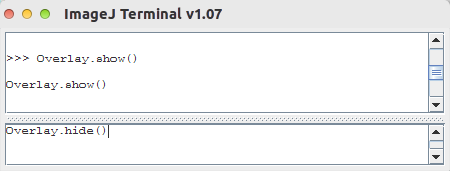
\includegraphics[width=0.8\textwidth]{macro_interpreter}
    \caption[The macro interpreter]{The macro interpreter allows to run single macro commands.}
    \label{macro_interpreter}
\end{figure}

\newpage

\section{Excercises}

\begin{ExerciseList}
\Exercise{{\bf Clearing the log window}}
\label{ex_2_1}

The command {\tt print("\textbackslash \textbackslash Clear")} clears the log window. Modify the macro in Listing \ref{lst:hello_world_log_window}, so that the log window is cleared before the message is written. Run the modified macro multiple times and compare the behaviour of the original macro with the behaviour of the modified version.

\Exercise{{\bf Message dialog with a title}}
\label{ex_2_2}

Did you notice that the message window in figure \ref{dialog_window} does not have a title? Add a title by modifying Listing \ref{lst:hello_world_dialog}. In order to give it a title you need to add a parameter to the call of the {\tt showMessage()} command. The title needs to be the first parameter, the text to be displayed the second parameter.

\Exercise{{\bf Drawing a rectangle on an overlay}}
\label{ex_2_3}

Modify the macro in Listing \ref{lst:hello_world_image}! Draw a rectangle around the ''Hello World'' text onto the overlay! Use the command {\tt Overlay.drawRect(x, y, width, height)}. You need to find the value for {\tt x}, {\tt y}, {\tt width} and {\tt height}. You can use the menu item {\tt Image>>Overlay>>Remove Overlay} to clean the overlay between different trials. 

\Exercise{{\bf Recording commands}}
\label{ex_2_4}
In this exercise you will record a number of commands and apply them to another image. Open an example image. You can use {\tt File>>Open Samples>>Clown (14K)}. Now start the macro recorder and execute the following commands: 
\begin{itemize}
\item {\tt Process>>Smooth}
\item {\tt Process>>Find Edges}
\item {\tt Edit>>Invert}
\end{itemize}
Press the {\tt Create} button of the macro recorder to create the macro. Now close the image, open another example image, for example {\tt File>>Open Samples>>Bridge (174K)} and run the recorded macro on this image.

\newpage

\section{Answers}

\Answer[ref={ex_2_1}]

{\bf Clearing the log window}

\begin{listing}[H]
\begin{minted}[frame=lines, linenos]{java}
print("\\Clear");
print("Hello World!");
\end{minted}
\caption{In the modified macro the log window is cleared before the text is written.}
\label{lst:clear_log_window}
\end{listing}

In the original version of the macro each time you run the macro a line with the output text is added to the log window. In the new version the log window is cleared before the text is written so that the result is a log window with the output text in the first line each time you run the macro.

\Answer[ref={ex_2_2}]

{\bf Message dialog with a title}

\begin{listing}[H]
\begin{minted}[frame=lines]{java}
showMessage("Greetings", "Hello World!");
\end{minted}
\caption{The dialog of the hello world message will now have a title.}
\label{lst:dialog_with_title}
\end{listing}

Running the macro should produce something similar to figure \ref{dialog_with_title}.

\begin{center}
    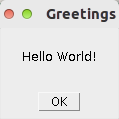
\includegraphics[width=0.2\textwidth]{dialog_with_title}
    \captionof{figure}{The dialog now has the title ''Greetings''.}
    \label{dialog_with_title}
\end{center}

\Answer[ref={ex_2_3}]

{\bf Drawing a rectangle on an overlay}

\begin{listing}[H]
\begin{minted}[frame=lines, linenos]{java}
setFont("Serif", 40, " antialiased");
setColor("#ffc800");
Overlay.drawRect(100,50,300,100);
Overlay.drawString("Hello World!", 126, 128, 0.0);
Overlay.show();
\end{minted}
\caption{A rectangle is drawn around the message.}
\label{lst:hello_world_rectangle}
\end{listing}

Running the macro should yield a result similar to figure \ref{hello_world_rect_result}.

\begin{center}
    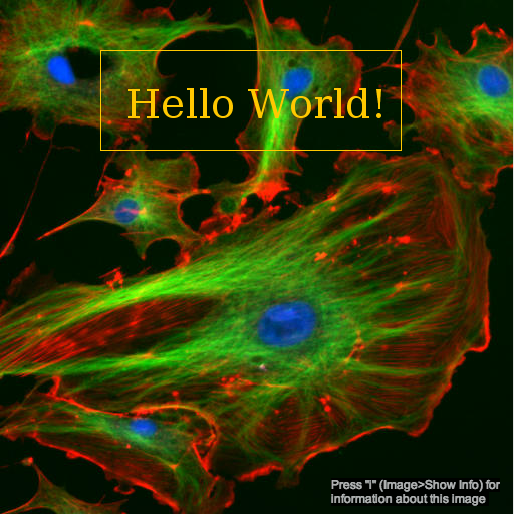
\includegraphics[width=0.4\textwidth]{Hello_World_Rect_Result}
    \captionof{figure}{The result of drawing a rectangle around the message.}
    \label{hello_world_rect_result}
\end{center}

\Answer[ref={ex_2_4}]

{\bf Recording commands}

\begin{listing}[H]
\begin{minted}[frame=lines, linenos]{java}
run("Smooth");
run("Find Edges");
run("Invert");
\end{minted}
\caption{The sequence of recorded commands should look like this.}
\label{lst:recorded_commands}
\end{listing}

Figure \ref{recorded_commands_result} shows the result of applying the recorded macro to the {\tt bridge} example image.

\begin{center}
    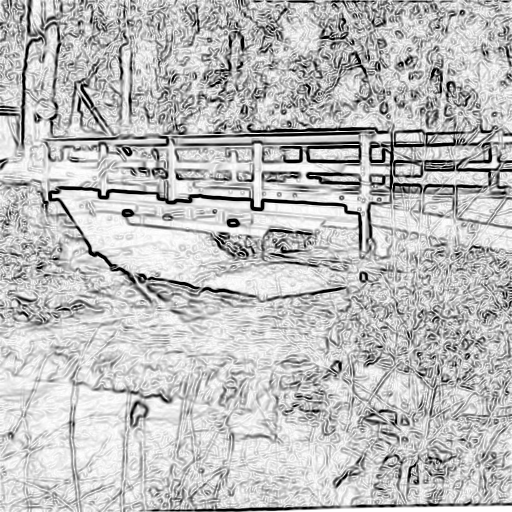
\includegraphics[width=0.6\textwidth]{bridge}
    \captionof{figure}{The result image after the recorded macro has been applied to it.}
    \label{recorded_commands_result}
\end{center}

\end{ExerciseList}


